\documentclass[10pt]{beamer}

\usetheme[nosectionslide]{m}

% camel case
\renewcommand{\mthemetitleformat}{}

\definecolor{mDarkRed}{HTML}{8F0129}
\definecolor{mGreen}{HTML}{0E8740}

\definecolor{BrickRed}{HTML}{B6321C}
\definecolor{DarkOrchid}{HTML}{A4538A}
\definecolor{ForestGreen}{HTML}{009B55}
\definecolor{Goldenrod}{HTML}{897E4D}

\setbeamercolor{alerted text}{fg=mGreen}
\setbeamertemplate{bibliography item}[text]

\setbeamertemplate{footnote}{\hangpara{2em}{1}\makebox[2em][l]{\insertfootnotemark}\footnotesize\insertfootnotetext\par}


\usepackage[scale=2]{ccicons}

\usepackage{cmap}           % Mapeamento de caracteres especiais no PDF
\usepackage{lmodern}        % Usa fonte Latin Modern
\usepackage[T1]{fontenc}    % Seleção de codificação de fonte
\usepackage[utf8]{inputenc} % Codificação do arquivo (conversão automática dos acentos)
\usepackage[brazil]{babel}  % Idioma para hifenização e tradução de vários elementos
\usepackage{makeidx}        % Criação de índice
\usepackage{hyperref}       % Formatação do índice
\usepackage{lastpage}       % Usado pela Ficha catalográfica
\usepackage{indentfirst}    % Indenta o primeiro parágrafo de cada seção
\usepackage{graphicx}       % Inclusão de gráficos
\usepackage{booktabs}       % Formatação de tabelas
% -------------------------------------------------------------------------------------------------
% Para citações
% \usepackage[brazilian,hyperpageref]{backref} % Páginas com as citações na bibliografia
\usepackage[alf]{abntex2cite} % Citações padrão ABNT (alfanumérico)
% -------------------------------------------------------------------------------------------------
% Pacotes opcionais
\usepackage{nomencl}        % Para criar uma lista de símbolos
\usepackage{acro}           % Para usar acrônimos e abreviaturas
\usepackage{tikz}           % Para fazer figuras, diagramas e gráficos integrados e elegantes
\usepackage{pgfplots}       % Usa o pacote tikz para fazer gráficos muito melhores que os do Excel
\usepackage{pgfplotstable}  % Para gerar tabelas automaticamente a partir de arquivos com dados
\usepackage{filecontents}   % Para colocar o conteúdo de um arquivo dentro de um arquivo tex
\usepackage{todonotes}      % Para criar anotações durante o desenvolvimento do texto
%\usepackage{multirow}       % Permite fazer tabelas com múltiplas linhas
\let\newfloat=\undefined    % Workaround para usar o pacote algorithm
\usepackage{algorithm}      % Para escrever algoritmos
\usepackage{algpseudocode}
\usepackage{pifont}
% \usepackage{clrscode}       % Para escrever algoritmos
% \usepackage{clrscode3e}     % Para escrever algoritmos; mais simples que os pacotes acima
\usepackage{pdfpages}        % Para incluir a folha de aprovação assinada em PDF
\usepackage{amsmath}
\usepackage{amsfonts}
\usepackage{subcaption}
\newcolumntype{P}[1]{>{\centering\arraybackslash}m{#1}} 

\usepackage{tablefootnote}
\usepackage{adjustbox}
\usepackage{changepage}
\usepackage{color}


\captionsetup{labelformat=empty,labelsep=none}


\makeatletter
\newcommand\footnoteref[1]{\protected@xdef\@thefnmark{\ref{#1}}\@footnotemark}
\makeatother

\DeclareMathOperator*{\argmin}{arg\,min}
\DeclareMathOperator*{\argmax}{arg\,max}


\title{Análise de desempenho para o banco de dados MariaDB}
\subtitle{}
\date{17 de julho de 2015}
\author[Treviso]{Cristiano Daitx Ribeiro\\Igor Antunes Fogaça\\Marcos Vinícius Treviso\\}
\institute{Banco de Dados II - Universidade Federal do Pampa}
\titlegraphic{\hfill
\includegraphics[height=1.25cm]{img/unipampa_logo.png}}

\begin{document}

\maketitle


\begin{frame}
  \frametitle{Roteiro}
  % \setbeamertemplate{section in toc}[mine]
  % \tableofcontents[hideallsubsections]

  \begin{itemize}

    \item Introdução
    
    \begin{itemize}
      \item[\ ] MariaDB
      \item[\ ] Índices
    \end{itemize}


    \item Ambiente

    \item Resultados

    \item Avaliação

    \item Conclusão

  \end{itemize}

\end{frame}



\begin{frame}
  \frametitle{Roteiro}
  % \setbeamertemplate{section in toc}[mine]
  % \tableofcontents[hideallsubsections]

  \begin{itemize}

    \item Introdução
    
    \begin{itemize}
      \item[\ ] MariaDB
      \item[\ ] Índices
    \end{itemize}


    \item[\color{gray}{$\bullet$}] \textcolor{gray}{Ambiente}

    \item[\color{gray}{$\bullet$}] \textcolor{gray}{Resultados}

    \item[\color{gray}{$\bullet$}] \textcolor{gray}{Avaliação}

    \item[\color{gray}{$\bullet$}] \textcolor{gray}{Conclusão}

  \end{itemize}

\end{frame}



\section{Introdução}

\begin{frame}[fragile]
  \frametitle{MariaDB}

    \begin{itemize}
      \item Sistema de Gerenciamento de Banco de Dados Relacional
      \begin{itemize}
        \item[-] Funcionalidade e substituição para o MySQL
        \item[-] Autores originais do MySQL
        \item[-] Aprimoramentos de recursos, otmizações
        \item[-] Criado pelo próprio criador do MySQL: Michael Widenius
      \end{itemize}

    \end{itemize}

  
    \begin{figure}[htb]
    \begin{center}
        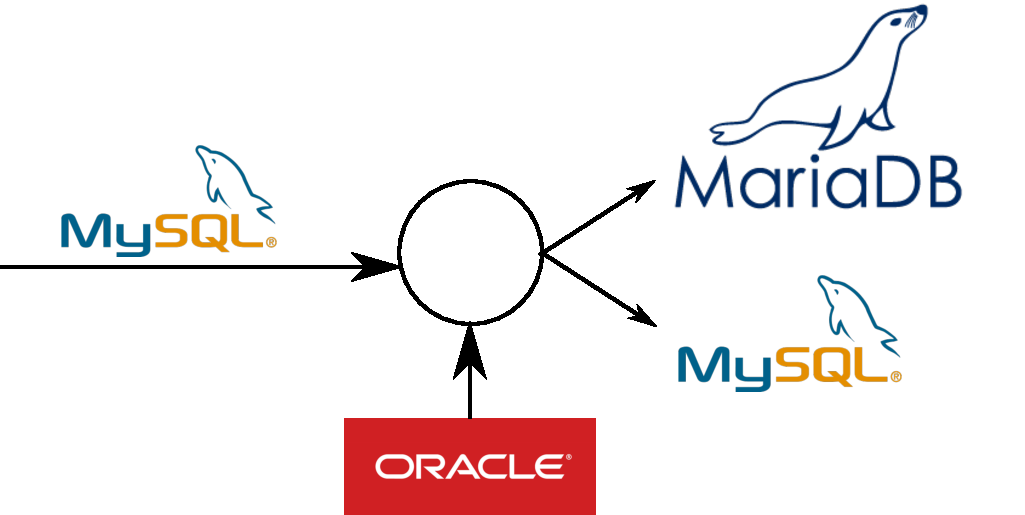
\includegraphics[scale=0.5]{img/mariadb.pdf}
    \end{center}
  \end{figure}

\end{frame}




\begin{frame}[fragile]
  \frametitle{Índices}

    \begin{itemize}

    \item Árvore B

      \begin{itemize}
        \item[-] >, >=, =, <=, <, !=, BETWEEN
        \item[-] LIKE (apenas com prefixo)
      \end{itemize}

    \item[\ ] \ 
    \item Hash
    \begin{itemize}
      \item[-] >, >=, =, <=, <, !=
      \item[-] LIKE sem substrings
    \end{itemize}

    \item[\ ] \ 
    \item Árvore R
    \begin{itemize}
      \item[-] >, >=, =, <=, <, !=, BETWEEN
      \item[-] LIKE
      \item[-] Apenas campos NOT NULL
    \end{itemize}

    \end{itemize}



\end{frame}




\begin{frame}
  \frametitle{Roteiro}
  % \setbeamertemplate{section in toc}[mine]
  % \tableofcontents[hideallsubsections]

  \begin{itemize}

    \item[\color{gray}{$\bullet$}] \textcolor{gray}{Introdução}
    
    \begin{itemize}
      \item[\ ] \textcolor{gray}{MariaDB}
      \item[\ ] \textcolor{gray}{Índices}
    \end{itemize}


    \item Ambiente

    \item[\color{gray}{$\bullet$}] \textcolor{gray}{Resultados}

    \item[\color{gray}{$\bullet$}] \textcolor{gray}{Avaliação}

    \item[\color{gray}{$\bullet$}] \textcolor{gray}{Conclusão}


  \end{itemize}

\end{frame}



\begin{frame}[fragile]
  \frametitle{Ambiente}

 \begin{itemize}
      \item Notebook HP Pavilion dv6 
    \end{itemize}

    \begin{table}[!htb]
    \footnotesize
    \centering
    \begin{tabular}{ll}
      \toprule
      \textbf{Processador} & Intel i7-2670QM 2.20GHz  \\
      \textbf{Memória Principal} & 8 GB RAM DDR3 1333 MHz \\
      \textbf{Disco} & TOSHIBA MK1059GS 1 TB \\
      \textbf{Cache} & L3 Cache 6 MB \\
      \bottomrule
    \end{tabular}
    % \caption{Dados dos \textit{córpus}} \label{tab:dadoscorpus}
    \end{table}

  \begin{itemize}
    \item SGBD: MariaDB versão 10.0.20
    \item Engine de armazenamento: InnoDB 
  \end{itemize}
  
\end{frame}


\begin{frame}[fragile]
  \frametitle{Ambiente}

  \begin{itemize}
    \item Banco de dados
    \begin{itemize}
      \item[-] 5 tabelas com tamanho: $10^2, 10^3, 10^4, 10^5, 10^6$
      \item[-] Índice primário sobre campo $id$
      \item[-] Índice secundário sobre campo $pais$
      \item[-] Índice secundário composto sobre campos $nome, sobrenome$
      \item[-] Índices utilizando árvore B
    \end{itemize}
  \end{itemize}

  \begin{table}[!htb]
    \footnotesize
    \centering
    \begin{tabular}{cccccc}
      \toprule
      \textbf{\underline{idrobos} (int)} & \textbf{nome (int)}  & \textbf{sobrenome (int)}  & \textbf{pais (int)} & \textbf{senha (int)} & \textbf{idade (int)}  \\
       \midrule
      $[0, |T|]$ & $[0, 10^3]$ & $[0, 10^3]$ & $[0, 250]$ & $[0, 10^6]$ & $[0, 10^2]$ \\
      \bottomrule
    \end{tabular}
   \end{table}


   \begin{itemize}
    
      \item Média de 15 tempos de execução
      \item Eliminação da cache:
      \begin{verbatim}
      SET GLOBAL query_cache_size, query_cache_type = 0, 0;
      \end{verbatim}
      \item Atribuição aleatória para população das tabelas
    
  \end{itemize}

\end{frame}



\begin{frame}
  \frametitle{Roteiro}
  % \setbeamertemplate{section in toc}[mine]
  % \tableofcontents[hideallsubsections]

  \begin{itemize}

    \item[\color{gray}{$\bullet$}] \textcolor{gray}{Introdução}
    
    \begin{itemize}
      \item[\ ] \textcolor{gray}{MariaDB}
      \item[\ ] \textcolor{gray}{Índices}
    \end{itemize}


    \item[\color{gray}{$\bullet$}] \textcolor{gray}{Ambiente}

    \item Resultados

    \item[\color{gray}{$\bullet$}] \textcolor{gray}{Avaliação}

    \item[\color{gray}{$\bullet$}] \textcolor{gray}{Conclusão}

  \end{itemize}

\end{frame}



\section{Resultados}

\begin{frame}[fragile]
  \frametitle{Resultados}


  \begin{itemize}
  \item Conjunto f) coleção 1:

  \footnotesize{\item \textbf{Consulta 1: } \texttt{SELECT * FROM tabela WHERE iP != valor}}

  \item  \footnotesize{\textbf{Consulta 2: } \texttt{SELECT * FROM tabela WHERE iS != valor}}

   \item \footnotesize{\textbf{Consulta 3: } \texttt{SELECT * FROM tabela WHERE iC1 != valor}}
  
   \item \footnotesize{\textbf{Consulta 4: } \texttt{SELECT * FROM tabela WHERE iC2 != valor}}
  
   \item \footnotesize{\textbf{Consulta 5: } \texttt{SELECT * FROM tabela WHERE ni != valor}}

   \item[\ ] \

  \end{itemize}

\begin{adjustwidth}{-2em}{-2em}


 \begin{table}[!htb]
    \footnotesize
    \centering
    \begin{tabular}{lccccc}
      \toprule
      \textbf{Consulta} & \textbf{100}  & \textbf{1000}  & \textbf{10000} & \textbf{100000} & \textbf{1000000}  \\
      \midrule
      * | iP != valor  & 0.78 (100)  &  0.71 (999)  & 2.95 (9998)  & 4.92 (99997) & 4.14 (999998)  \\
      * | iS != valor  & 0.74 (96)  &  0.74 (997)  & 7.77 (9940)  & 12.68 (99631) & 29.96 (995929)  \\
      * | iC1 != valor & 0.74 (99)  &  0.70 (999) & 5.34 (9989)  & 10.18 (99894) & 24.25 (999017)  \\
      * | iC2 != valor & 0.59 (98)  &  0.57 (999)  & 0.46 (9989)  & 0.66 (99897) & 0.45 (999012)  \\
      * | ni != valor  & 0.58 (100)  &  0.53 (1000) & 0.50 (9999)  & 0.62 (99999) & 0.43 (999997)  \\
      \bottomrule
    \end{tabular}
    \caption{Tempo de execução (ms) - Quantidade de tuplas afetadas} 
    \end{table}

\end{adjustwidth}
\end{frame}



\begin{frame}
  \frametitle{Resultados}
  % \setbeamertemplate{section in toc}[mine]
  % \tableofcontents[hideallsubsections]

\begin{adjustwidth}{-3em}{-3em}
\vspace{-1em}

  \begin{figure}[!htb]
  \label{fig:grafico_dados}
  \begin{center}
  \begin{tikzpicture}[scale=1]
    \begin{axis}[
      mlineplot,
      width=1\textwidth,
      height=0.75\textwidth,
      xmode=log,
      ymode=normal,
      ymin=0,
      xtick=data,
      ticks=both,
      xlabel=Tamanho,
      ylabel=Tempo de execução (ms),
      legend pos=north west,
      legend style={draw=none},
    ]
    \addplot table [x=tamanho,y=consulta1,header=true] {resultados1.txt};
    \addlegendentry{* | iP != valor}
    \addplot+[DarkOrchid] table [x=tamanho,y=consulta2,header=true] {resultados1.txt};
    \addlegendentry{* | iS != valor}
    \addplot+[ForestGreen] table [x=tamanho,y=consulta3,header=true] {resultados1.txt};
    \addlegendentry{* | iC1 != valor}
    \addplot+[BrickRed] table [x=tamanho,y=consulta4,header=true] {resultados1.txt};
    \addlegendentry{* | iC2 != valor}
    \addplot+[Goldenrod,mark=o] table [x=tamanho,y=consulta5,header=true] {resultados1.txt};
    \addlegendentry{* | ni != valor}
  \end{axis}
  \end{tikzpicture}
\end{center}
\end{figure}
  

\end{adjustwidth}
\end{frame}






\begin{frame}
  \frametitle{Resultados}
  % \setbeamertemplate{section in toc}[mine]
  % \tableofcontents[hideallsubsections]

\begin{adjustwidth}{-3em}{-3em}
\vspace{-1em}

  \begin{figure}[!htb]
  \label{fig:grafico_dados}
  \begin{center}
  \begin{tikzpicture}[scale=1]
    \begin{axis}[
      mbarplot,
      width=1\textwidth,
      height=0.75\textwidth,
      xmode=log,
      ymode=log,
      ymin=0,
      xtick=data,
      ticks=both,
      xlabel=Tamanho,
      ylabel=Quantidade de tuplas afetadas,
      legend pos=north west,
      legend style={draw=none},
    ]
    \addplot table [x=tamanho,y=consulta1,header=true] {resultados1x.txt};
    \addlegendentry{* | iP != valor}
    \addplot table [x=tamanho,y=consulta2,header=true] {resultados1x.txt};
    \addlegendentry{* | iS != valor}
    \addplot table [x=tamanho,y=consulta3,header=true] {resultados1x.txt};
    \addlegendentry{* | iC1 != valor}
    \addplot table [x=tamanho,y=consulta4,header=true] {resultados1x.txt};
    \addlegendentry{* | iC2 != valor}
    \addplot table [x=tamanho,y=consulta5,header=true] {resultados1x.txt};
    \addlegendentry{* | ni != valor}
  \end{axis}
  \end{tikzpicture}
\end{center}
\end{figure}
  

\end{adjustwidth}
\end{frame}




\begin{frame}[fragile]
  \frametitle{Resultados}


  \begin{itemize}
  \item Conjunto f) coleção 2:

  \footnotesize{\item \textbf{Consulta 1: } \texttt{SELECT * FROM tabela WHERE iP = valor AND iS = valor}}

  \item  \footnotesize{\textbf{Consulta 2: } \texttt{SELECT * FROM tabela WHERE iS = valor AND iP = valor}}

   \item \footnotesize{\textbf{Consulta 3: } \texttt{SELECT iP FROM tabela WHERE iP = valor AND iS = valor}}
  
   \item \footnotesize{\textbf{Consulta 4: } \texttt{SELECT iP FROM tabela WHERE iS = valor AND iP = valor}}
  
   \item \footnotesize{\textbf{Consulta 5: } \texttt{SELECT iP,iS FROM tabela WHERE iP = valor AND iS = valor}}

   \item \footnotesize{\textbf{Consulta 6: } \texttt{SELECT iP,iS FROM tabela WHERE iS = valor AND iP = valor}}

   \item[\ ] \

  \end{itemize}

\begin{adjustwidth}{-2em}{-2em}

 \begin{table}[!htb]
    \footnotesize
    \centering
    \begin{tabular}{lccccc}
      \toprule
      \textbf{Consulta} & \textbf{100}  & \textbf{1000}  & \textbf{10000} & \textbf{100000} & \textbf{1000000}  \\
      \midrule
      Consulta 1  & 0.65 (0.2)  &  2.56 (0.1)  & 8.59 (0.1)  & 48.46 (0.2) & 444.57 (0.2)  \\
      Consulta 2  & 0.64 (0.2)  &  2.58 (0.2)  & 15.43 (0.3)  & 50.44 (0.3) & 445.45 (0.1)  \\
      Consulta 3 & 0.56 (0.1)  &  0.96 (0.1) & 8.62 (0.2)  & 38.47 (0.2) & 279.38 (0.2)  \\
      Consulta 4 & 0.58 (0.1)  &  1.04 (0.1)  & 8.52 (0.2)  & 47.44 (0.3) & 280.41 (0.2)  \\
      Consulta 5 & 0.64 (0.2)  &  1.10 (0.2) & 8.41 (0.2)  & 37.43 (0.2) & 282.51 (0.3)  \\
      Consulta 6  & 0.66 (0.2)  &  1.01 (0.1) & 8.46 (0.2)  & 38.16 (0.2) & 279.42 (0.4)  \\
      \bottomrule
    \end{tabular}
    \caption{Tempo de execução (ms) - Quantidade de tuplas afetadas} 
    \end{table}

\end{adjustwidth}
\end{frame}



\begin{frame}
  \frametitle{Resultados}
  % \setbeamertemplate{section in toc}[mine]
  % \tableofcontents[hideallsubsections]

\begin{adjustwidth}{-3em}{-3em}
\vspace{-1em}

  \begin{figure}[!htb]
  \label{fig:grafico_dados}
  \begin{center}
  \begin{tikzpicture}[scale=1]
    \begin{axis}[
      mlineplot,
      width=1\textwidth,
      height=0.75\textwidth,
      xmode=log,
      ymode=log,
      ymin=0.3,
      % ymax=1.3,
      xtick=data,
      ticks=both,
      xlabel=Tamanho,
      ylabel=Tempo de execução (ms),
      legend pos=north west,
      legend style={draw=none},
    ]

    \addplot table [x=tamanho,y=consulta1,header=true] {resultados2.txt};
    \addlegendentry{\scriptsize{* | iP = valor AND iS = valor}}
    \addplot+[DarkOrchid] table [x=tamanho,y=consulta2,header=true] {resultados2.txt};
    \addlegendentry{\scriptsize{* | iS = valor AND iP = valor}}
    \addplot table [x=tamanho,y=consulta3,header=true] {resultados2.txt};
    \addlegendentry{\scriptsize{iP | iP = valor AND iS = valor}}
    \addplot+[ForestGreen] table [x=tamanho,y=consulta4,header=true] {resultados2.txt};
    \addlegendentry{\scriptsize{iP | iS = valor AND iP = valor}}
    \addplot+[Goldenrod,mark=o] table [x=tamanho,y=consulta5,header=true] {resultados2.txt};
    \addlegendentry{\scriptsize{iP,iS | iP = valor AND iS = valor}}
    \addplot+[BrickRed,mark=x] table [x=tamanho,y=consulta6,header=true] {resultados2.txt};
    \addlegendentry{\scriptsize{iP,iS | iS = valor AND iP = valor}}

  \end{axis}
  \end{tikzpicture}
\end{center}
\end{figure}
  

\end{adjustwidth}
\end{frame}






\begin{frame}
  \frametitle{Resultados}
  % \setbeamertemplate{section in toc}[mine]
  % \tableofcontents[hideallsubsections]

\begin{adjustwidth}{-3em}{-3em}
\vspace{-1em}

  \begin{figure}[!htb]
  \label{fig:grafico_dados}
  \begin{center}
  \begin{tikzpicture}[scale=1]
    \begin{axis}[
      mbarplot,
      width=1\textwidth,
      height=0.75\textwidth,
      xmode=log,
      ymode=normal,
      ymin=0,
      ymax=1,
      xtick=data,
      ticks=both,
      xlabel=Tamanho,
      ylabel=Quantidade de tuplas afetadas,
      legend pos=north west,
      legend style={draw=none},
    ]
    \addplot table [x=tamanho,y=consulta1,header=true] {resultados2x.txt};
    \addlegendentry{\scriptsize{* | iP = valor AND iS = valor}}
    \addplot table [x=tamanho,y=consulta2,header=true] {resultados2x.txt};
    \addlegendentry{\scriptsize{* | iS = valor AND iP = valor}}
    \addplot table [x=tamanho,y=consulta3,header=true] {resultados2x.txt};
    \addlegendentry{\scriptsize{iP | iP = valor AND iS = valor}}
    \addplot table [x=tamanho,y=consulta4,header=true] {resultados2x.txt};
    \addlegendentry{\scriptsize{iP | iS = valor AND iP = valor}}
    \addplot table [x=tamanho,y=consulta5,header=true] {resultados2x.txt};
    \addlegendentry{\scriptsize{iP,iS | iP = valor AND iS = valor}}
    \addplot table [x=tamanho,y=consulta6,header=true] {resultados2x.txt};
    \addlegendentry{\scriptsize{iP,iS | iS = valor AND iP = valor}}
  \end{axis}
  \end{tikzpicture}
\end{center}
\end{figure}
  

\end{adjustwidth}
\end{frame}




\begin{frame}
  \frametitle{Roteiro}
  % \setbeamertemplate{section in toc}[mine]
  % \tableofcontents[hideallsubsections]

  \begin{itemize}

    \item[\color{gray}{$\bullet$}] \textcolor{gray}{Introdução}
    
    \begin{itemize}
      \item[\ ] \textcolor{gray}{MariaDB}
      \item[\ ] \textcolor{gray}{Índices}
    \end{itemize}


    \item[\color{gray}{$\bullet$}] \textcolor{gray}{Ambiente}

    \item[\color{gray}{$\bullet$}] \textcolor{gray}{Resultados}

    \item Avaliação

    \item[\color{gray}{$\bullet$}] \textcolor{gray}{Conclusão}

  \end{itemize}

\end{frame}



\section{Avaliação}

\begin{frame}[fragile]
  \frametitle{Avaliação}

    \begin{itemize}
      \item \textbf{Consulta 1: } \texttt{SELECT * FROM tabela WHERE iP != valor}
      \begin{itemize}
        \item[-] Índice primário
        \item[-] Operação de desigualdade
        \item[-] Todos os dados da tabela
      \end{itemize}

      \item[\ ] \ 

    \end{itemize}

     \begin{table}[!htb]
    \footnotesize
    \centering
    \begin{tabular}{lccccc}
      \toprule
      \textbf{Tamanho} & \textbf{Tipo de Acesso}  & \textbf{Chaves Possíveis}  & \textbf{Chave Usada} & \textbf{Linhas} & \textbf{Extra}  \\
      \midrule
      $10^2$  & variável  &  primária  & primária  & 99      & where  \\
      $10^3$  & variável  &  primária  & primária  & 997     & where  \\
      $10^4$  & variável  &  primária  & primária  & 5053    & where  \\
      $10^5$  & variável  &  primária  & primária  & 47096   & where  \\
      $10^6$  & variável  &  primária  & primária  & 479274  & where  \\

      \bottomrule
    \end{tabular}
    % \caption{Dados dos \textit{córpus}} \label{tab:dadoscorpus}
    \end{table}
   

\end{frame}


\begin{frame}[fragile]
  \frametitle{Avaliação}

    \begin{itemize}
      \item \textbf{Consulta 2: } \texttt{SELECT * FROM tabela WHERE iS != valor}
      \begin{itemize}
        \item[-] Indíce secundário
        \item[-] Operação de desigualdade
        \item[-] Todos os dados da tabela
      \end{itemize}

      \item[\ ] \ 

    \end{itemize}

     \begin{table}[!htb]
    \footnotesize
    \centering
    \begin{tabular}{lccccc}
      \toprule
      \textbf{Tamanho} & \textbf{Tipo de Acesso}  & \textbf{Chaves Possíveis}  & \textbf{Chave Usada} & \textbf{Linhas} & \textbf{Extra}  \\
      \midrule
      $10^2$  & linear  &  secundária  & nenhuma  & 100     & where  \\
      $10^3$  & linear  &  secundária  & nenhuma  & 1000    & where  \\
      $10^4$  & linear  &  secundária  & nenhuma  & 10104   & where  \\
      $10^5$  & linear  &  secundária  & nenhuma  & 93912   & where  \\
      $10^6$  & linear  &  secundária  & nenhuma  & 958268  & where  \\

      \bottomrule
    \end{tabular}
    % \caption{Dados dos \textit{córpus}} \label{tab:dadoscorpus}
    \end{table}

    % A full table scan is done for the table (all rows are read). This is bad if the table is large and the table is joined against a previous table! This happens when the optimizer could not find any usable index to access rows.
   

\end{frame}


\begin{frame}[fragile]
  \frametitle{Avaliação}

    \begin{itemize}
      \item \textbf{Consulta 3: } \texttt{SELECT * FROM tabela WHERE iC1 != valor}
      \begin{itemize}
        \item[-] Primeiro elemento do indíce composto
        \item[-] Operação de desigualdade
        \item[-] Todos os dados da tabela
      \end{itemize}

      \item[\ ] \ 

    \end{itemize}

     \begin{table}[!htb]
    \footnotesize
    \centering
    \begin{tabular}{lccccc}
      \toprule
      \textbf{Tamanho} & \textbf{Tipo de Acesso}  & \textbf{Chaves Possíveis}  & \textbf{Chave Usada} & \textbf{Linhas} & \textbf{Extra}  \\
      \midrule
      $10^2$  & linear  &  composta$^{1}$  & nenhuma  & 100     & where  \\
      $10^3$  & linear  &  composta$^{1}$  & nenhuma  & 1000    & where  \\
      $10^4$  & linear  &  composta$^{1}$  & nenhuma  & 10104   & where  \\
      $10^5$  & linear  &  composta$^{1}$  & nenhuma  & 93912   & where  \\
      $10^6$  & linear  &  composta$^{1}$  & nenhuma  & 958268  & where  \\

      \bottomrule
    \end{tabular}
    % \caption{Dados dos \textit{córpus}} \label{tab:dadoscorpus}
    \end{table}

\end{frame}



\begin{frame}[fragile]
  \frametitle{Avaliação}

    \begin{itemize}
      \item \textbf{Consulta 4: } \texttt{SELECT * FROM tabela WHERE iC2 != valor}
      \begin{itemize}
        \item[-] Segundo elemento do indíce composto
        \item[-] Operação de desigualdade
        \item[-] Todos os dados da tabela
      \end{itemize}

      \item[\ ] \ 

    \end{itemize}

     \begin{table}[!htb]
    \footnotesize
    \centering
    \begin{tabular}{lccccc}
      \toprule
      \textbf{Tamanho} & \textbf{Tipo de Acesso}  & \textbf{Chaves Possíveis}  & \textbf{Chave Usada} & \textbf{Linhas} & \textbf{Extra}  \\
      \midrule
      $10^2$  & linear  &  nenhuma  & nenhuma  & 100     & where  \\
      $10^3$  & linear  &  nenhuma  & nenhuma  & 1000    & where  \\
      $10^4$  & linear  &  nenhuma  & nenhuma  & 10104   & where  \\
      $10^5$  & linear  &  nenhuma  & nenhuma  & 93912   & where  \\
      $10^6$  & linear  &  nenhuma  & nenhuma  & 958268  & where  \\

      \bottomrule
    \end{tabular}
    % \caption{Dados dos \textit{córpus}} \label{tab:dadoscorpus}
    \end{table}

\end{frame}


\begin{frame}[fragile]
  \frametitle{Avaliação}

    \begin{itemize}
      \item \textbf{Consulta 5: } \texttt{SELECT * FROM tabela WHERE ni != valor}
      \begin{itemize}
        \item[-] Sem índice
        \item[-] Operação de desigualdade
        \item[-] Todos os dados da tabela
      \end{itemize}

      \item[\ ] \ 

    \end{itemize}

     \begin{table}[!htb]
    \footnotesize
    \centering
    \begin{tabular}{lccccc}
      \toprule
      \textbf{Tamanho} & \textbf{Tipo de Acesso}  & \textbf{Chaves Possíveis}  & \textbf{Chave Usada} & \textbf{Linhas} & \textbf{Extra}  \\
      \midrule
      $10^2$  & linear  &  nenhuma  & nenhuma  & 100     & where  \\
      $10^3$  & linear  &  nenhuma  & nenhuma  & 1000    & where  \\
      $10^4$  & linear  &  nenhuma  & nenhuma  & 10104   & where  \\
      $10^5$  & linear  &  nenhuma  & nenhuma  & 93912   & where  \\
      $10^6$  & linear  &  nenhuma  & nenhuma  & 958268  & where  \\

      \bottomrule
    \end{tabular}
    % \caption{Dados dos \textit{córpus}} \label{tab:dadoscorpus}
    \end{table}

\end{frame}




\begin{frame}[fragile]
  \frametitle{Avaliação}

  \begin{itemize}

    \item Foi usado índice apenas na consulta sobre a chave primária

    \item Por que linear?
      \begin{itemize}
        \item[-] Operação de desigualdade
        \item[-] Distribuição uniforme e aleatória 
      \end{itemize}

    \item Por que nenhuma chave possível para a Consulta 4 (segundo elemento do índice composto)?
    \begin{itemize}
        \item[-] MariaDB ordena pelo primeiro elemento, e depois pelo segundo
        \item[-] \texttt{ return (a.first < b.first) ? true : (a.second < b.second)}
      \end{itemize}

    \item Por que as linhas previstas não ficaram parecidas com o encontrado?
    \begin{itemize}
      \item[-] Estimativa de custos
      \item[-] Atribuição pseudoaleatória 
    \end{itemize}

  \end{itemize}

  \begin{equation}
  n_r - \dfrac{n_r}{V(A,r)} \nonumber
  \end{equation}

\end{frame}


\begin{frame}[fragile]
  \frametitle{Avaliação}

  \begin{itemize}

    \item \textbf{Tempo de execução:}

    \item Consulta 1 (chave primária)
      \begin{itemize}
        \item[-] Utilizou o índice primário $\to$ Tempo de execução baixo
      \end{itemize}

    \item Consulta 2 (chave secundária)
      \begin{itemize}
        \item[-] Não utilizou o índice secundário $\to$ Tempo de execução alto conforme o tamanho da tabela cresce 
      \end{itemize}

    \item Consulta 3 (primeiro elemento da chave composta)
      \begin{itemize}
        \item[-] Não utilizou o índice composto
        \item[-] Crescimento semelhante a Consulta 2
      \end{itemize}

    \item Consulta 4 (segundo elemento da chave composta)
      \begin{itemize}
        \item[-] Não utilizou o índice composto
        \item[-] Busca linear
      \end{itemize}

    \item Consulta 5 (primeiro elemento da chave composta)
      \begin{itemize}
        \item[-] Busca linear
        \item[-] Comportamento muito semelhante a Consulta 4
      \end{itemize}


  \end{itemize}


\end{frame}


\begin{frame}[fragile]
  \frametitle{Avaliação}

    \begin{itemize}
      \item \textbf{Consulta 1: } \footnotesize{\texttt{SELECT * FROM tabela WHERE iP = valor AND iS = valor}}
      \begin{itemize}
        \item[-] Índice primário e secundário
        \item[-] Operação de AND sobre igualdade
        \item[-] Todos os dados da tabela
      \end{itemize}

    \end{itemize}

     \begin{table}[!htb]
    \footnotesize
    \centering
    \begin{tabular}{lccccc}
      \toprule
      \textbf{Tamanho} & \textbf{Tipo de Acesso}  & \textbf{Chaves Possíveis}  & \textbf{Chave Usada} & \textbf{Linhas} & \textbf{Extra}  \\
      \midrule
      $10^2$  & NULL  &  nenhuma  & nenhuma  & NULL  & impossível \\
      $10^3$  & NULL  &  nenhuma  & nenhuma  & NULL  & impossível \\
      $10^4$  & NULL  &  nenhuma  & nenhuma  & NULL  & impossível \\
      $10^5$  & NULL  &  nenhuma  & nenhuma  & NULL  & impossível \\
      $10^6$  & NULL  &  nenhuma  & nenhuma  & NULL  & impossível \\

      \bottomrule
    \end{tabular}
    % \caption{Dados dos \textit{córpus}} \label{tab:dadoscorpus}
    \end{table}
   
    \begin{itemize}
    \item Ímpossível $\to$ Só há uma chance de ocorrer
    \item Caso ocorra, é utilizado o índice primário
    \end{itemize}


\end{frame}




\begin{frame}[fragile]
  \frametitle{Avaliação}

    \begin{itemize}
      \item \textbf{Consulta 2: } \footnotesize{\texttt{SELECT * FROM tabela WHERE iS = valor AND iP = valor}}
      \begin{itemize}
        \item[-] Índice primário e secundário
        \item[-] Operação de AND sobre igualdade
        \item[-] Todos os dados da tabela
      \end{itemize}

    \end{itemize}

     \begin{table}[!htb]
    \footnotesize
    \centering
    \begin{tabular}{lccccc}
      \toprule
      \textbf{Tamanho} & \textbf{Tipo de Acesso}  & \textbf{Chaves Possíveis}  & \textbf{Chave Usada} & \textbf{Linhas} & \textbf{Extra}  \\
      \midrule
      $10^2$  & NULL  &  nenhuma  & nenhuma  & NULL  & impossível \\
      $10^3$  & NULL  &  nenhuma  & nenhuma  & NULL  & impossível \\
      $10^4$  & NULL  &  nenhuma  & nenhuma  & NULL  & impossível \\
      $10^5$  & NULL  &  nenhuma  & nenhuma  & NULL  & impossível \\
      $10^6$  & NULL  &  nenhuma  & nenhuma  & NULL  & impossível \\

      \bottomrule
    \end{tabular}
    % \caption{Dados dos \textit{córpus}} \label{tab:dadoscorpus}
    \end{table}
   
    \begin{itemize}
    \item Ímpossível $\to$ Só há uma chance de ocorrer
    \item Caso ocorra, é utilizado o índice primário
    \end{itemize}


\end{frame}



\begin{frame}[fragile]
  \frametitle{Avaliação}

    \begin{itemize}
      \item \textbf{Consulta 3: } \footnotesize{\texttt{SELECT iP FROM tabela WHERE iP = valor AND iS = valor}}
      \begin{itemize}
        \item[-] Índice primário e secundário
        \item[-] Operação de AND sobre igualdade
        \item[-] Apenas campo do índice primário
      \end{itemize}

    \end{itemize}

     \begin{table}[!htb]
    \footnotesize
    \centering
    \begin{tabular}{lccccc}
      \toprule
      \textbf{Tamanho} & \textbf{Tipo de Acesso}  & \textbf{Chaves Possíveis}  & \textbf{Chave Usada} & \textbf{Linhas} & \textbf{Extra}  \\
      \midrule
      $10^2$  & NULL  &  nenhuma  & nenhuma  & NULL  & impossível \\
      $10^3$  & NULL  &  nenhuma  & nenhuma  & NULL  & impossível \\
      $10^4$  & NULL  &  nenhuma  & nenhuma  & NULL  & impossível \\
      $10^5$  & NULL  &  nenhuma  & nenhuma  & NULL  & impossível \\
      $10^6$  & NULL  &  nenhuma  & nenhuma  & NULL  & impossível \\

      \bottomrule
    \end{tabular}
    % \caption{Dados dos \textit{córpus}} \label{tab:dadoscorpus}
    \end{table}
   
    \begin{itemize}
    \item Ímpossível $\to$ Só há uma chance de ocorrer
    \item Caso ocorra, é utilizado o índice primário
    \end{itemize}


\end{frame}



\begin{frame}[fragile]
  \frametitle{Avaliação}

    \begin{itemize}
      \item \textbf{Consulta 4: } \footnotesize{\texttt{SELECT iP FROM tabela WHERE iS = valor AND iP = valor}}
      \begin{itemize}
        \item[-] Índice primário e secundário
        \item[-] Operação de AND sobre igualdade
        \item[-] Apenas campo do índice primário
      \end{itemize}

    \end{itemize}

     \begin{table}[!htb]
    \footnotesize
    \centering
    \begin{tabular}{lccccc}
      \toprule
      \textbf{Tamanho} & \textbf{Tipo de Acesso}  & \textbf{Chaves Possíveis}  & \textbf{Chave Usada} & \textbf{Linhas} & \textbf{Extra}  \\
      \midrule
      $10^2$  & NULL  &  nenhuma  & nenhuma  & NULL  & impossível \\
      $10^3$  & NULL  &  nenhuma  & nenhuma  & NULL  & impossível \\
      $10^4$  & NULL  &  nenhuma  & nenhuma  & NULL  & impossível \\
      $10^5$  & NULL  &  nenhuma  & nenhuma  & NULL  & impossível \\
      $10^6$  & NULL  &  nenhuma  & nenhuma  & NULL  & impossível \\

      \bottomrule
    \end{tabular}
    % \caption{Dados dos \textit{córpus}} \label{tab:dadoscorpus}
    \end{table}
   
    \begin{itemize}
    \item Ímpossível $\to$ Só há uma chance de ocorrer
    \item Caso ocorra, é utilizado o índice primário
    \end{itemize}


\end{frame}



\begin{frame}[fragile]
  \frametitle{Avaliação}

    \begin{itemize}
      \item \textbf{Consulta 5: } \footnotesize{\texttt{SELECT iP,iS FROM tabela WHERE iP = valor AND iS = valor}}
      \begin{itemize}
        \item[-] Índice primário e secundário
        \item[-] Operação de AND sobre igualdade
        \item[-] Apenas campo do índice primário e do secundário
      \end{itemize}

    \end{itemize}

     \begin{table}[!htb]
    \footnotesize
    \centering
    \begin{tabular}{lccccc}
      \toprule
      \textbf{Tamanho} & \textbf{Tipo de Acesso}  & \textbf{Chaves Possíveis}  & \textbf{Chave Usada} & \textbf{Linhas} & \textbf{Extra}  \\
      \midrule
      $10^2$  & NULL  &  nenhuma  & nenhuma  & NULL  & impossível \\
      $10^3$  & NULL  &  nenhuma  & nenhuma  & NULL  & impossível \\
      $10^4$  & NULL  &  nenhuma  & nenhuma  & NULL  & impossível \\
      $10^5$  & NULL  &  nenhuma  & nenhuma  & NULL  & impossível \\
      $10^6$  & NULL  &  nenhuma  & nenhuma  & NULL  & impossível \\

      \bottomrule
    \end{tabular}
    % \caption{Dados dos \textit{córpus}} \label{tab:dadoscorpus}
    \end{table}
   
    \begin{itemize}
    \item Ímpossível $\to$ Só há uma chance de ocorrer
    \item Caso ocorra, é utilizado o índice primário
    \end{itemize}


\end{frame}



\begin{frame}[fragile]
  \frametitle{Avaliação}

    \begin{itemize}
      \item \textbf{Consulta 6: } \footnotesize{\texttt{SELECT iP,iS FROM tabela WHERE iS = valor AND iP = valor}}
      \begin{itemize}
        \item[-] Índice primário e secundário
        \item[-] Operação de AND sobre igualdade
        \item[-] Apenas campo do índice primário e do secundário
      \end{itemize}

    \end{itemize}

     \begin{table}[!htb]
    \footnotesize
    \centering
    \begin{tabular}{lccccc}
      \toprule
      \textbf{Tamanho} & \textbf{Tipo de Acesso}  & \textbf{Chaves Possíveis}  & \textbf{Chave Usada} & \textbf{Linhas} & \textbf{Extra}  \\
      \midrule
      $10^2$  & NULL  &  nenhuma  & nenhuma  & NULL  & impossível \\
      $10^3$  & NULL  &  nenhuma  & nenhuma  & NULL  & impossível \\
      $10^4$  & NULL  &  nenhuma  & nenhuma  & NULL  & impossível \\
      $10^5$  & NULL  &  nenhuma  & nenhuma  & NULL  & impossível \\
      $10^6$  & NULL  &  nenhuma  & nenhuma  & NULL  & impossível \\

      \bottomrule
    \end{tabular}
    % \caption{Dados dos \textit{córpus}} \label{tab:dadoscorpus}
    \end{table}
   
    \begin{itemize}
    \item Ímpossível $\to$ Só há uma chance de ocorrer
    \item Caso ocorra, é utilizado o índice primário
    \end{itemize}


\end{frame}

\begin{frame}[fragile]
  \frametitle{Avaliação}

  \begin{itemize}

    \item Por que a ação foi ``impossível'' para todos?
    \begin{equation}
    P(iP, iS | T) = P(iP | T) \times P(iS | T) = \frac{1}{|T|} \times \frac{C(v_{iS}, T)}{|T|} \nonumber
    \end{equation}


    \item Caso dê a sorte de ocorrer
      \begin{itemize}
        \item[-] Primeiro é analisado o índice primário
        \item[-] Como ele é chave primária, é devolvido apenas um valor
      \end{itemize}

    \item[\ ] \ 

    \item Busca no índice primário

  \end{itemize}


\end{frame}




\begin{frame}
  \frametitle{Roteiro}
  % \setbeamertemplate{section in toc}[mine]
  % \tableofcontents[hideallsubsections]

  \begin{itemize}

    \item[\color{gray}{$\bullet$}] \textcolor{gray}{Introdução}
    
    \begin{itemize}
      \item[\ ] \textcolor{gray}{MariaDB}
      \item[\ ] \textcolor{gray}{Índices}
    \end{itemize}


    \item[\color{gray}{$\bullet$}] \textcolor{gray}{Ambiente}

    \item[\color{gray}{$\bullet$}] \textcolor{gray}{Resultados}

    \item[\color{gray}{$\bullet$}] \textcolor{gray}{Avaliação}

    \item Conclusão

  \end{itemize}

\end{frame}



\begin{frame}[fragile]
  \frametitle{Conclusão}

  \begin{itemize}

    \item A distribuição uniforme e aleatória afetou os resultados diretamente

    \item[\ ] \ 

    \item Nem sempre a criação de índices ajuda a melhorar o desempenho

    \item[\ ] \ 

    \item O comando EXPLAIN ajuda bastante a entender o plano de execução da consulta

    \item[\ ] \ 

    \item Alguns tempos de execução iniciais afetaram o resultado final para a primeira coleção 

  \end{itemize}

\end{frame}




\begin{frame}[fragile]
  \frametitle{Conclusão}

  \begin{itemize}

    \item Eficiência do MariaDB
    \begin{itemize}
      \item[-] Comparar com outros SGBDs
      \item[-] Analisar com dados de aplicações reais
    \end{itemize}

    \item[\ ] \ 

    \item Outros comandos
    \begin{itemize}
      \item[-] OR
      \item[-] ORDER BY
      \item[-] JOINS
    \end{itemize}

    \item[\ ] \ 

    \item Outras instruções
    \begin{itemize}
      \item[-] INSERT
      \item[-] UPDATE
      \item[-] DELETE
    \end{itemize}

  \end{itemize}

\end{frame}




% \section{Referências}

% \begin{frame}[allowframebreaks,noframenumbering]

%   \frametitle{Referências}
%   \bibliography{bibliografia,abntex2-modelo-references}

% \end{frame}


\begin{frame}[fragile]
  \frametitle{Referências}

  Página de documentação do MariaDB. Disponível em: \url{https://mariadb.com/kb/en/mariadb/}.

 \textbf{\\ \ }

CHEIRAN, J. F. Transparências de aulas de Banco de Dados II. Universidade Federal do Pampa, 2015. 


\end{frame}



\plain{Análise de desempenho para o banco de dados MariaDB \\ \ \\ \normalsize{Cristiano Daitx Ribeiro\\Igor Antunes Fogaça\\Marcos Vinícius Treviso} \\ \ \\ \ \\ {Banco de Dados II} \\ \ \\ \ \\ {\normalsize 17 de julho de 2015} \\ {\scriptsize Universidade Federal do Pampa}}




\end{document}
